During the duration of the dedicated photon run all SVT hybrids and APV25 
readout chips were configured to their nominal operating 
points~\cite{Jones:1069892} while all sensors were reverse-bias at 180~V.  The 
sensors were operated within a temperature range of  20 to 24$^\circ$C 
throughout the test run. Multiple calibration runs established a noise level of 60-68 
ADC counts ($\approx$ 750 - 850 electrons)  which was stable across all hybrids. With a linear gain up to $\approx 3$~MIPs, the 
cluster charge for hits associated with a track follow the characteristic Landau shape with a 
mean of about 25,500~e$^{-}$ as expected, see Fig.~\ref{fig:cluster_pulse}.
%This signal response gives a signal-to-noise ratio of about 25.5. 
\begin{figure}[h]
    % TODO: The pulse plot needs to be remade such that the x-axis is time 
	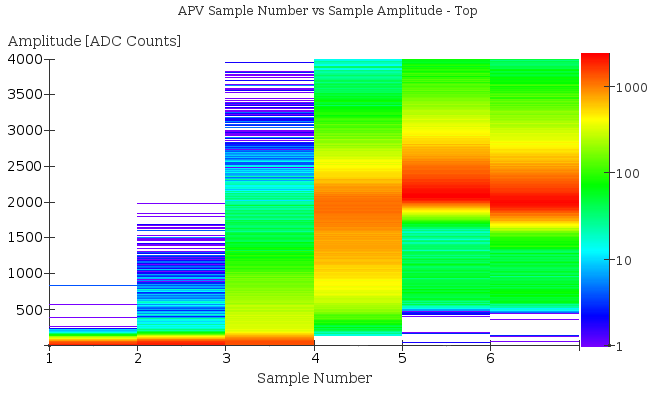
\includegraphics[width=0.49\textwidth]{test2012/svtperformance/svt_calib/08062012_run1351_samples_vs_amplitude.png}
	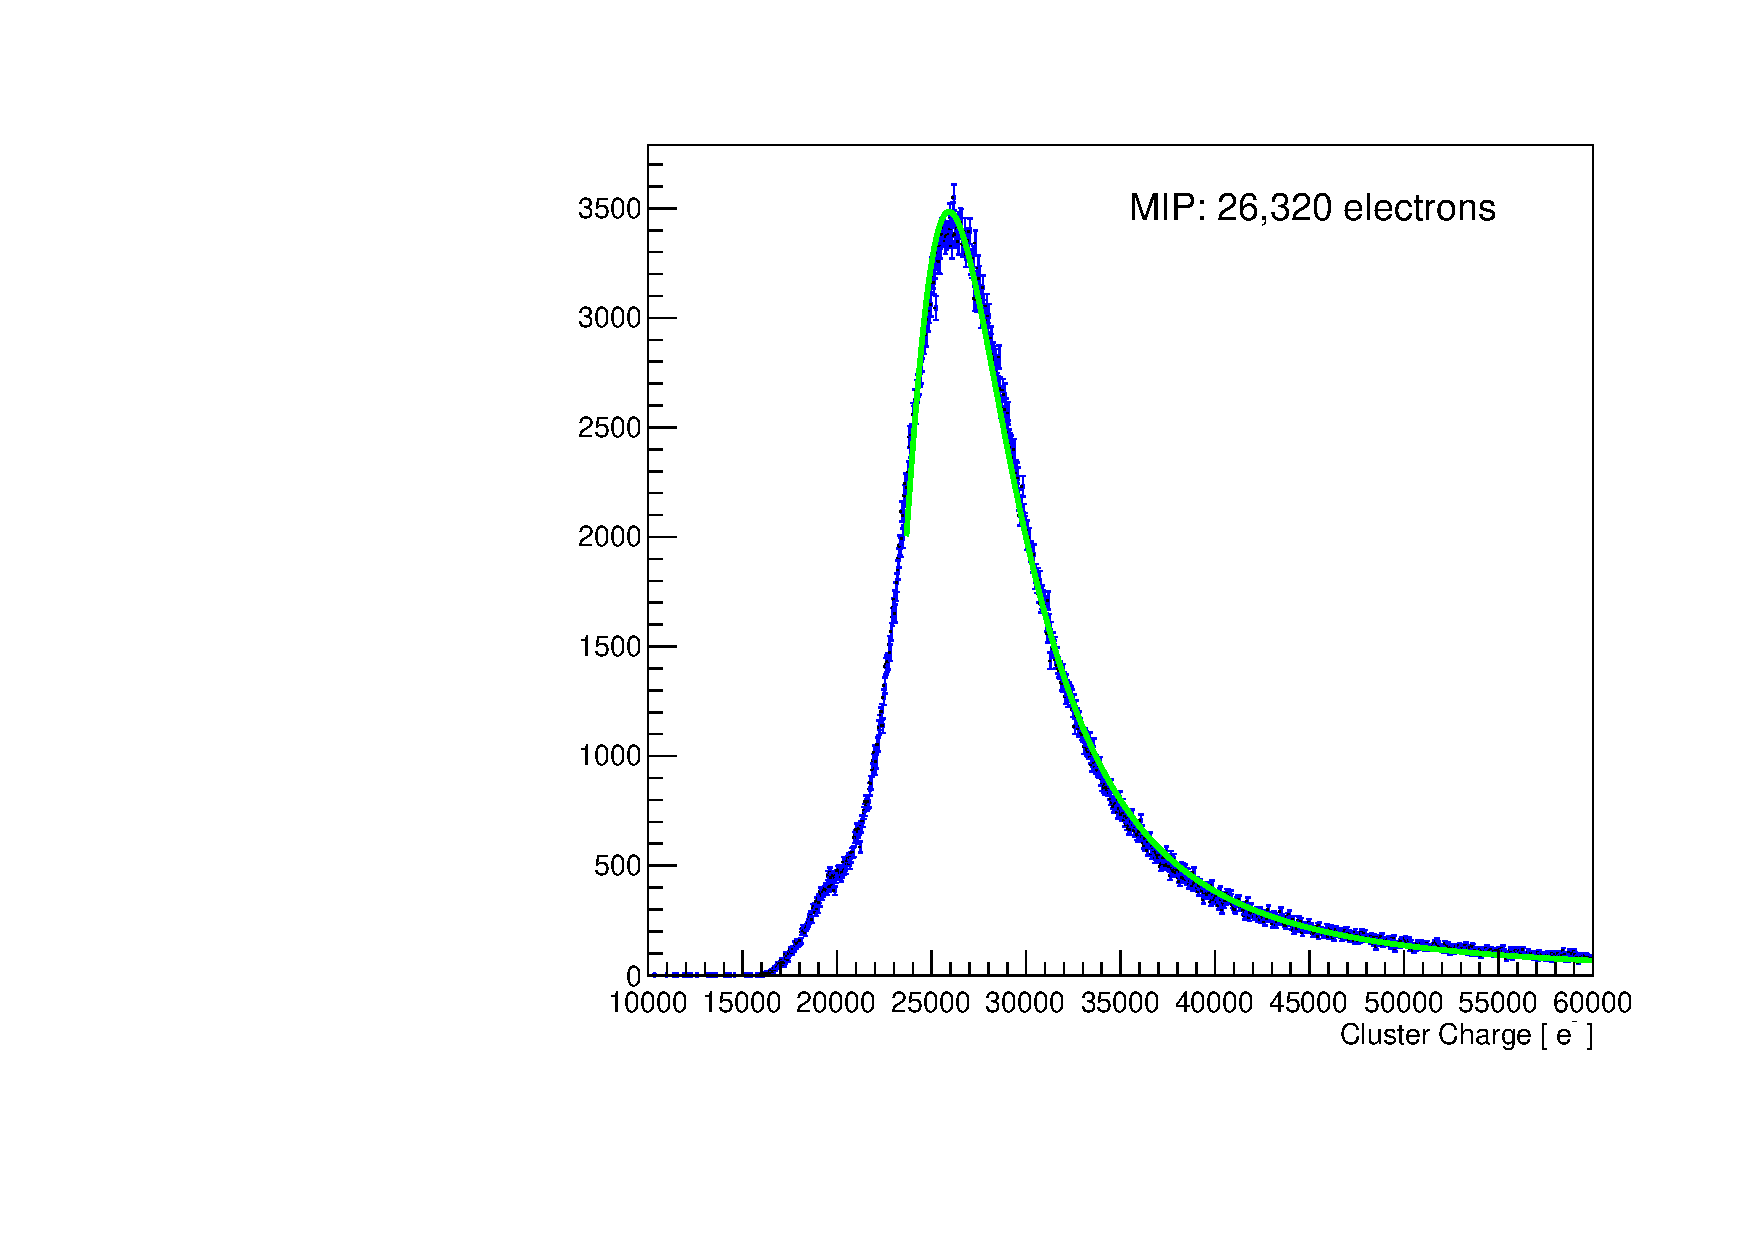
\includegraphics[width=0.49\textwidth]{test2012/svtperformance/svt_calib/run1351_mip_small.pdf}
    \caption{The six pedestal subtracted samples associated with a hit on a track 
             are shown on the left plot along with a distribution of the cluster
             charge exhibiting the characteristic Landau shape on the right. 
            }
	\label{fig:cluster_pulse}
\end{figure}


One of the important tests of the SVT was the operation of the APV25 chips in multi-peak readout mode 
discussed in Sec.~\ref{sec:svt}. The six samples of the APV25 pulse shaper output 
are fitted to an ideal $CR-RC$ function to extract the amplitude and the $t0$ of the hit. 
The typical pulse shape obtained is shown in Figure~\ref{fig:cluster_pulse} also demonstrates that the SVT was well timed in to the trigger with the rise of the pulse at the 3rd sampling point.
After clustering hits on a sensor, the hit time for each cluster is computed as the amplitude-weighted average of 
the fitted $t0$ channel times. The $t0$-resolution is studied by comparing the cluster hit time with the average of all cluster hit times, the ``track time''. Figure~\ref{fig:tracktime} shows the track time, with the expected jitter due to clock phase and trigger, and the residual to the individual cluster times. 
\begin{figure}[h]
%	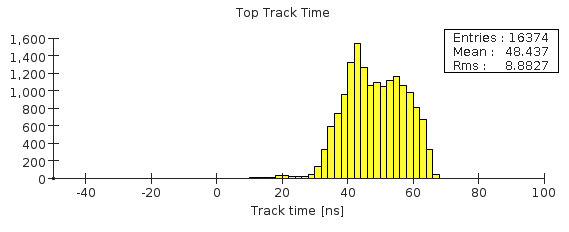
\includegraphics[width=0.7\textwidth]{test2012/svtperformance/track_time_top}
%	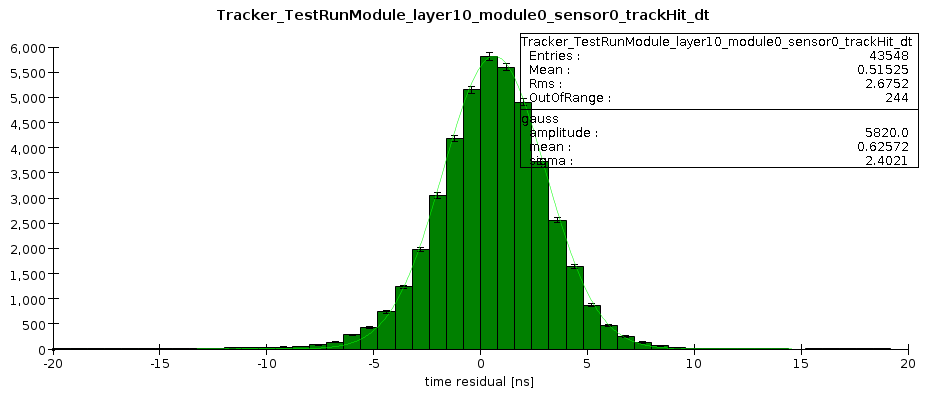
\includegraphics[width=0.7\textwidth]{test2012/svtperformance/timeres}
	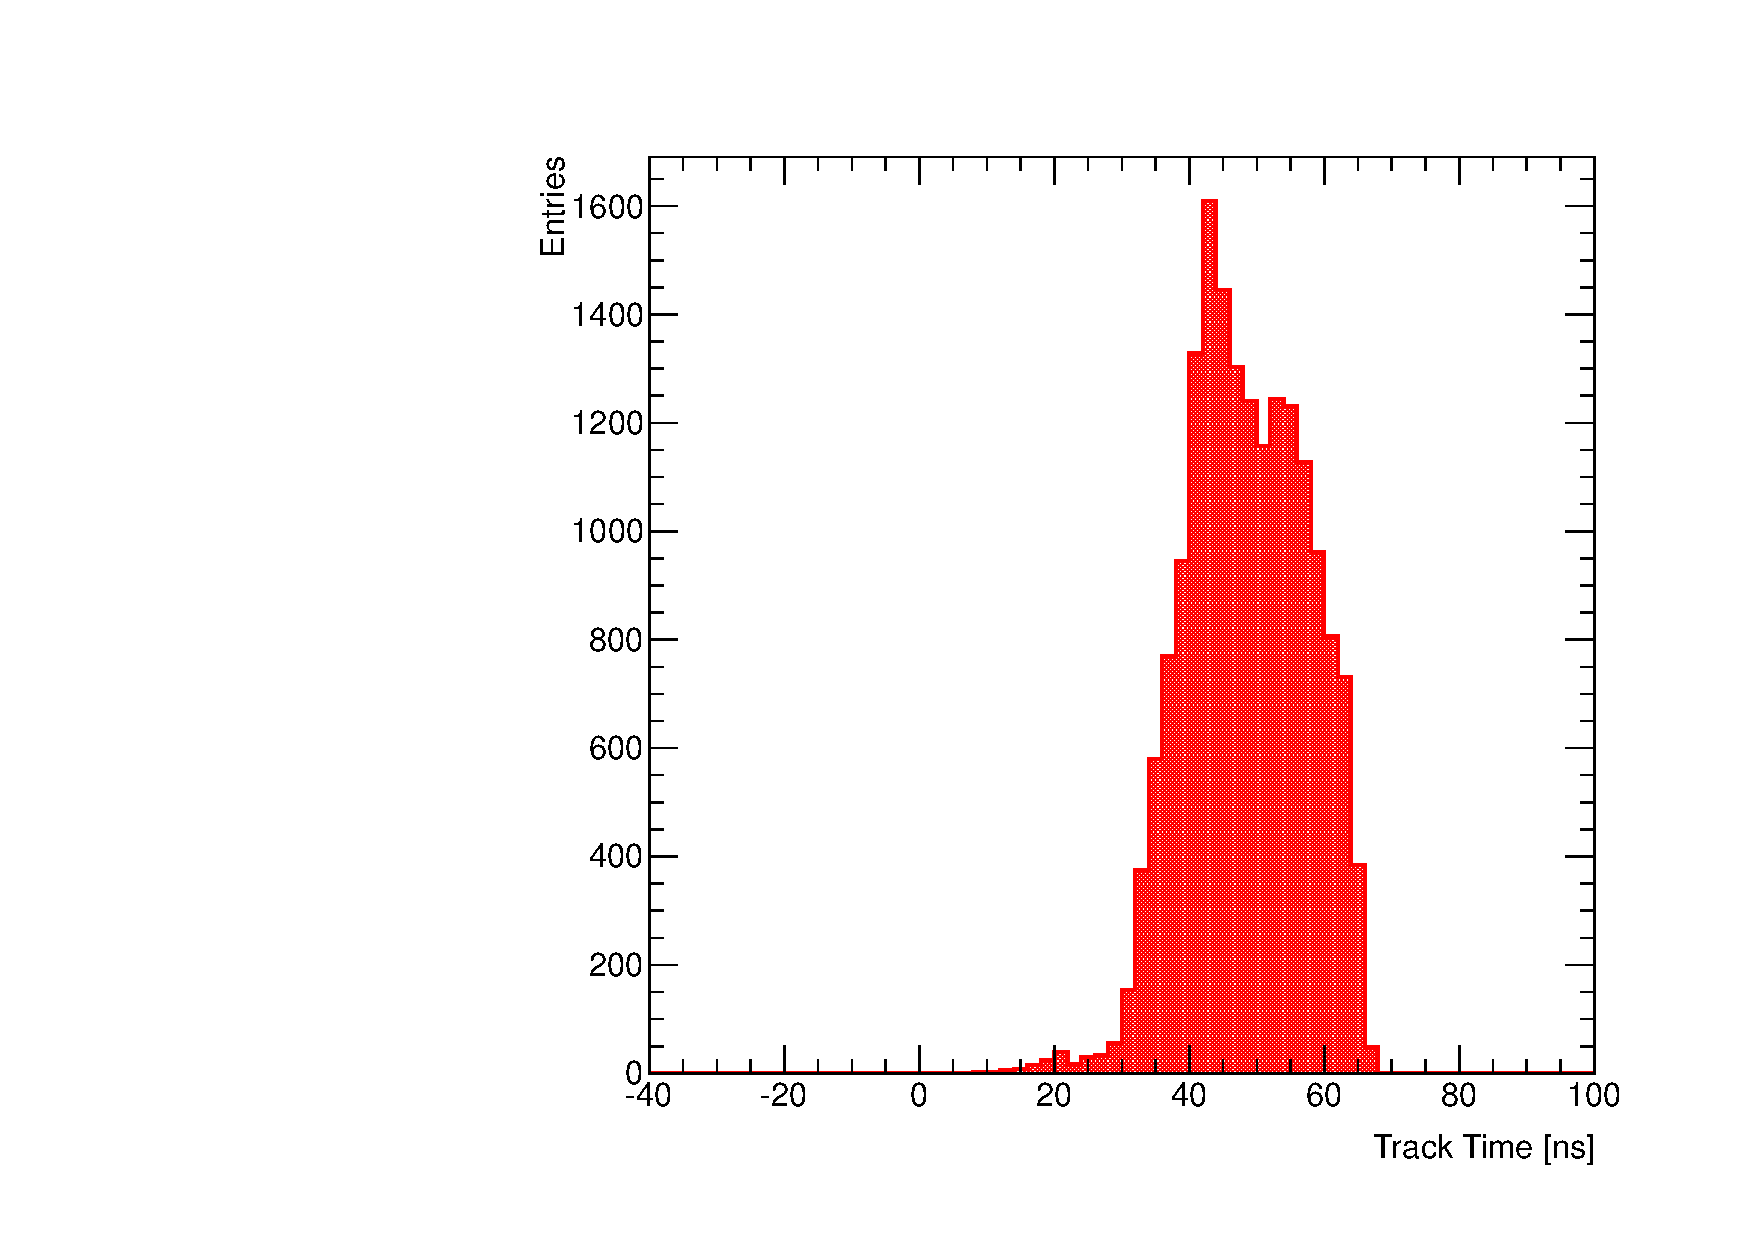
\includegraphics[width=0.49\textwidth]{test2012/svtperformance/top_track_time.pdf}
	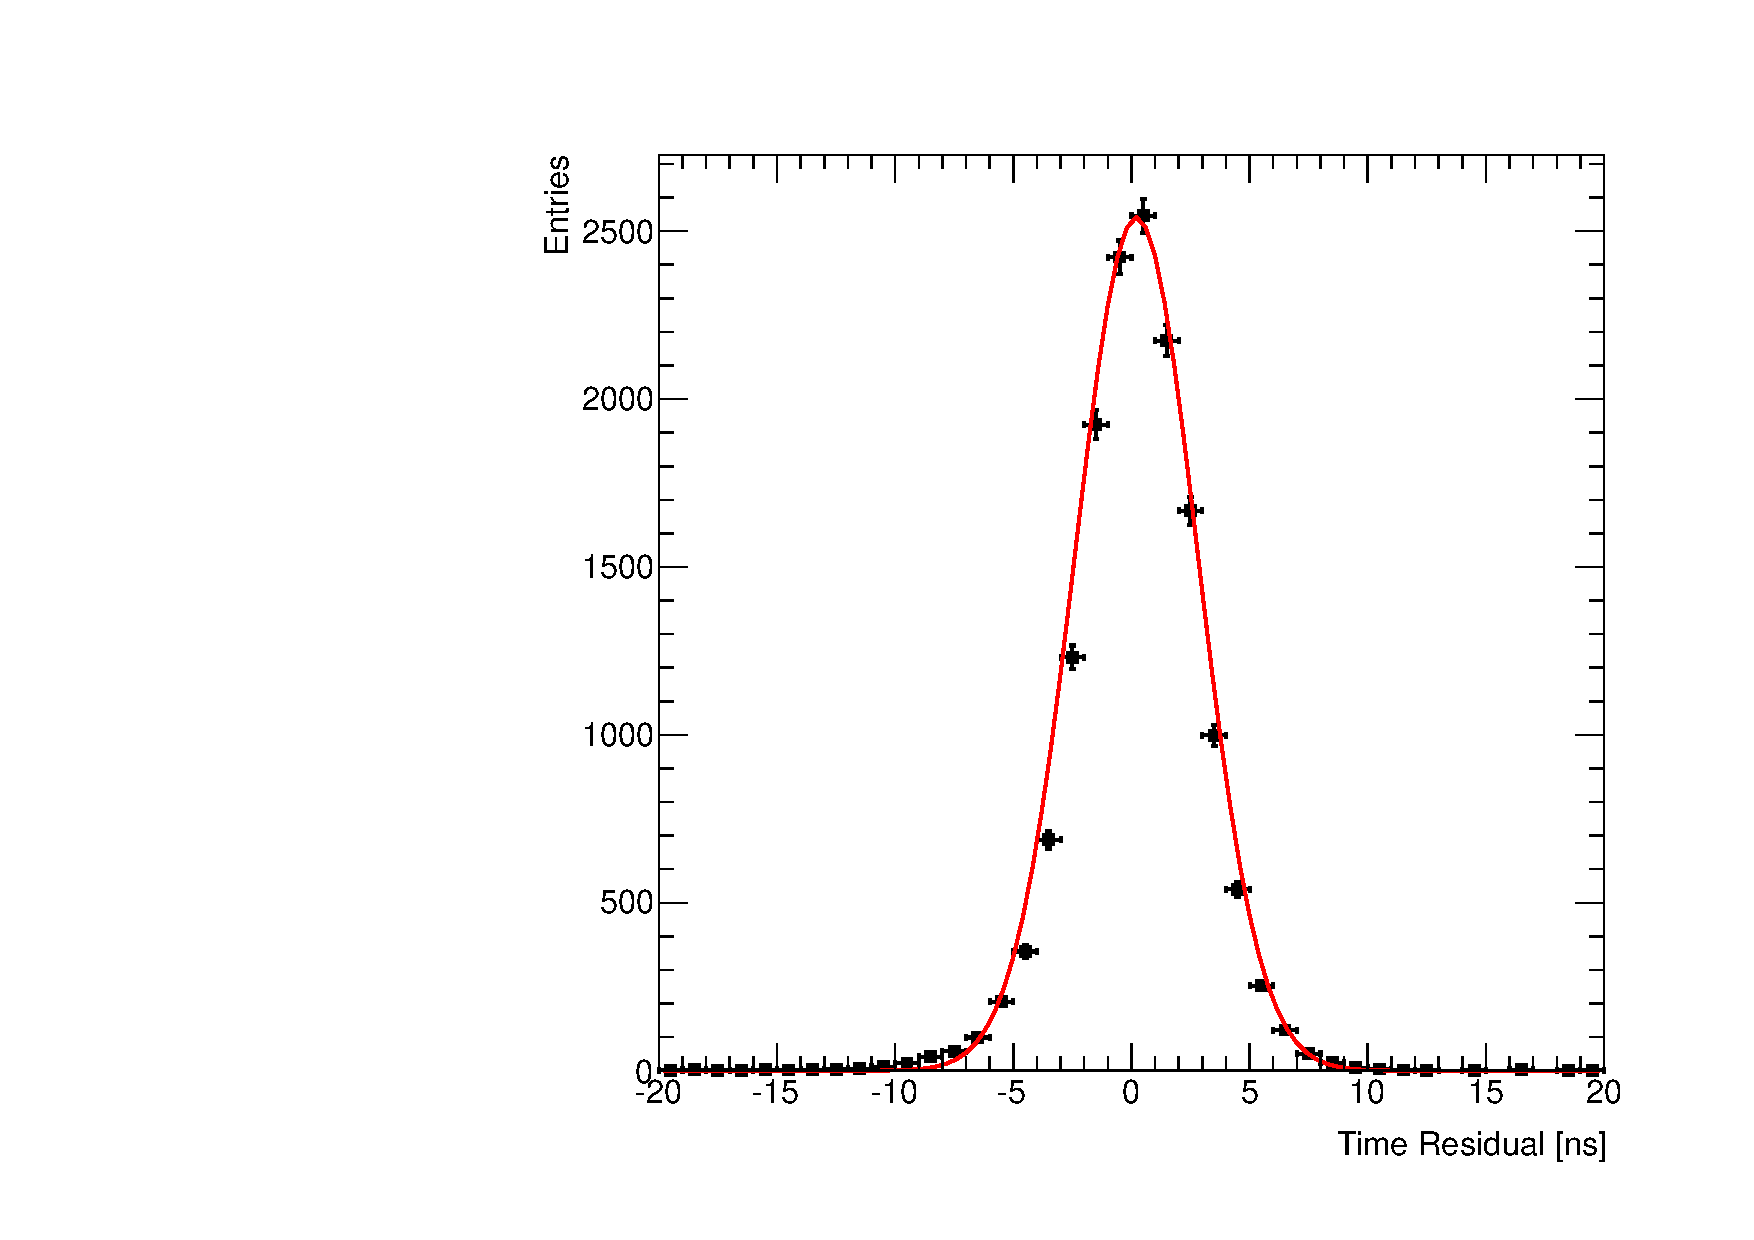
\includegraphics[width=0.49\textwidth]{test2012/svtperformance/t0_resolution.pdf}
	\caption{\small{Track time distribution (left) and cluster time residual (right). The 
	track time is measured relative to the APV25 clock. The width of the distribution is due to 
	trigger jitter (24~ns jitter in the tracker readout clock, plus 16~ns jitter in the trigger system). 
	The cluster time residual is for a representative sensor relative to the track time.}}
	\label{fig:tracktime}
\end{figure}
After correcting for offsets from each sensor (time-of-flight, clock phase) the extracted $t0$ resolution is 2.6~ns. This is somewhat worse than the $\approx 2$ ns resolution expected in Section~\ref{sec:performance} which we attribute to the true pulse shape differing from our idealized fit function; work is in progress to use the true pulse shape in the fit.
Reducing the APV25 pulse shaping time will also improve time resolution.
In short, these results show that we can achieve time resolution adequate for pileup rejection during electron running.


Throughout the duration of the test run, approximately 97\% of the 12,780 SVT 
channels were found to be operating normally. 
The fraction of dead or noisy channels varied from 2.4\% to 4.7\%; 
most of these were due to misconfigured readout chips (2--4 misconfigured chips out of 100 total) 
a known noisy half-module, and a couple of known noisy readout chips. 
These issues will be resolved for future running.

% The identified dead or noisy channels were largely attributed to a 
% known noisy half-module and a few noisy or misconfigured chips which will be resolved for future running. 
This resulted in occupancies and data rates that were higher than what were expected from simulation; 
the maximum data rate observed in the SVT was 4.1 MB/s.
However, after masking out all known noisy channels found during the commissioning of the SVT, good agreement 
between simulation and test run occupancies was achieved as shown on Figure~\ref{fig:data_rates_data_mc_cmp}.

\begin{figure}[h]
    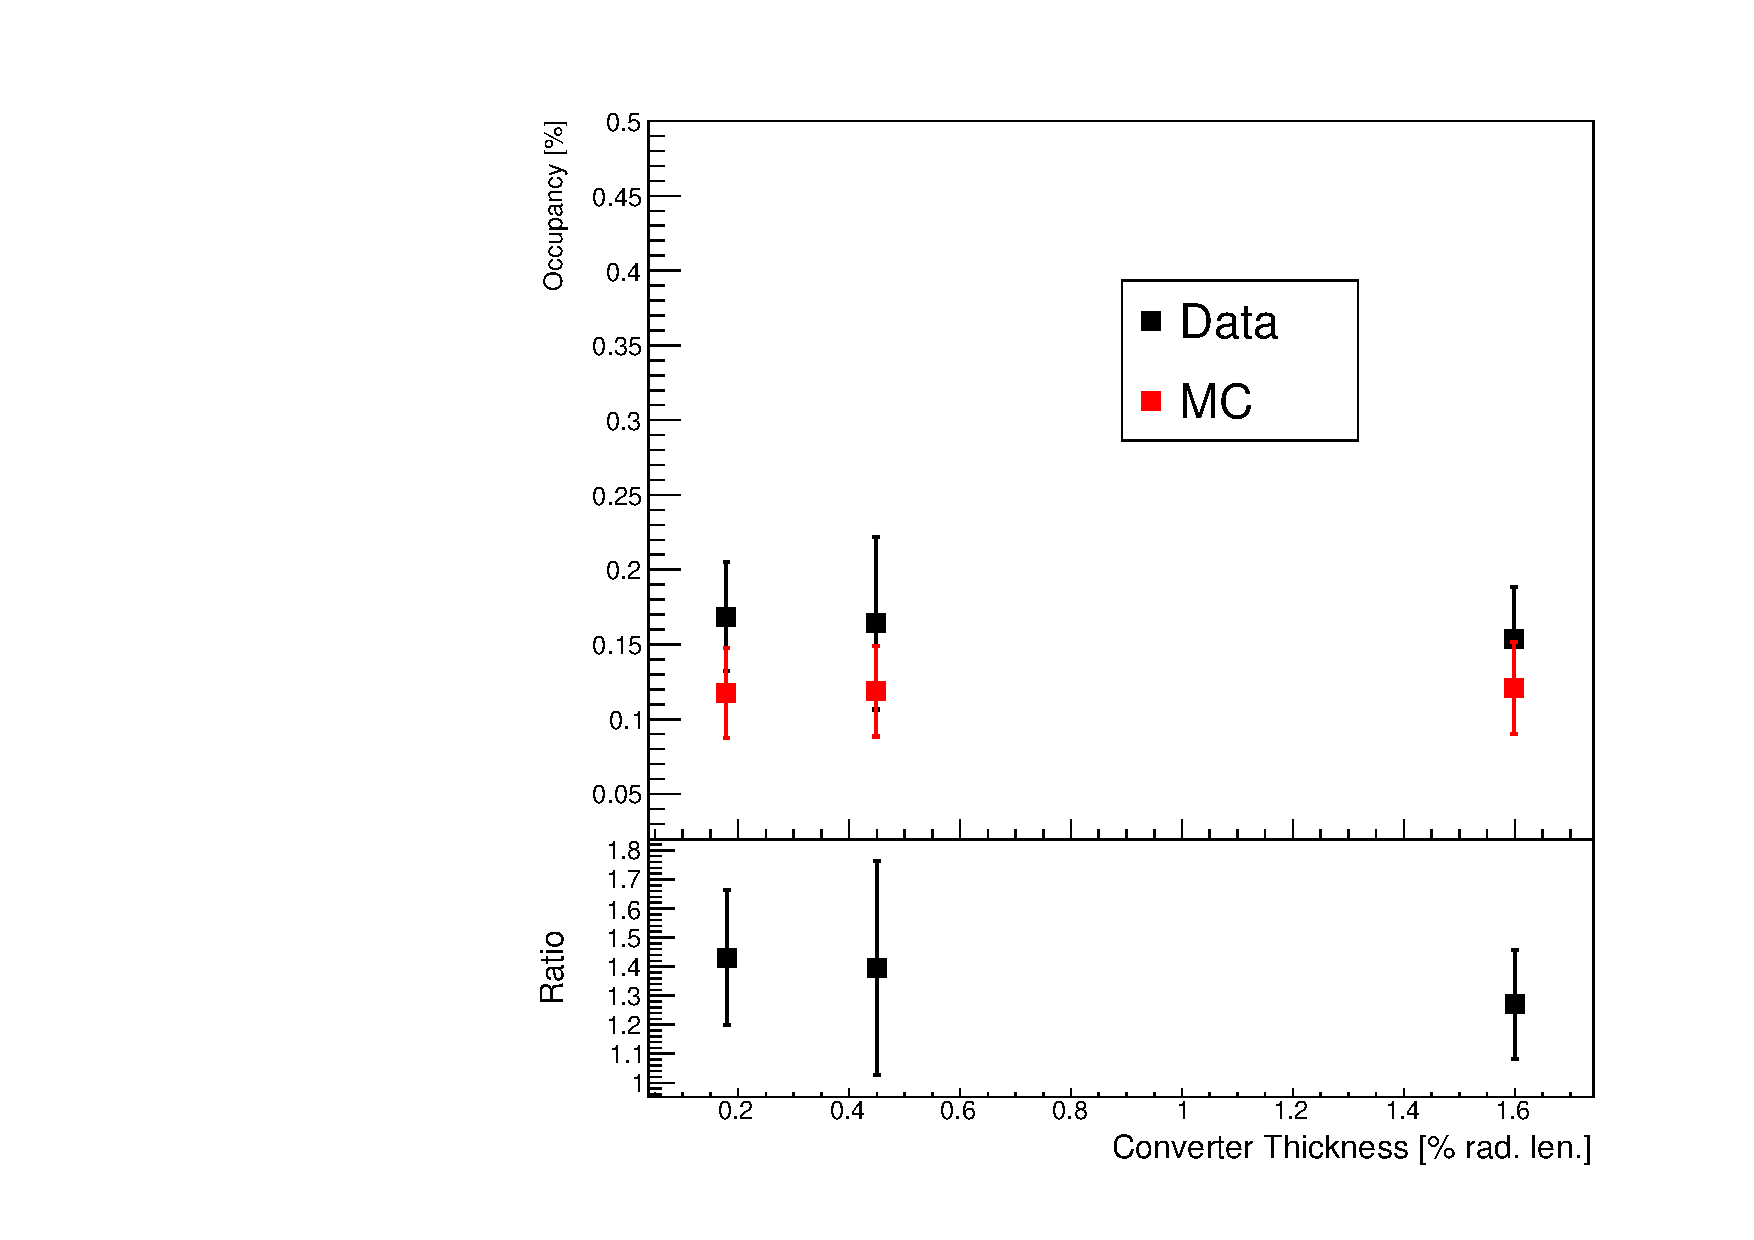
\includegraphics[width=0.49\textwidth]{test2012/svtperformance/daq/occupancy_vs_target_thick.pdf}
    % 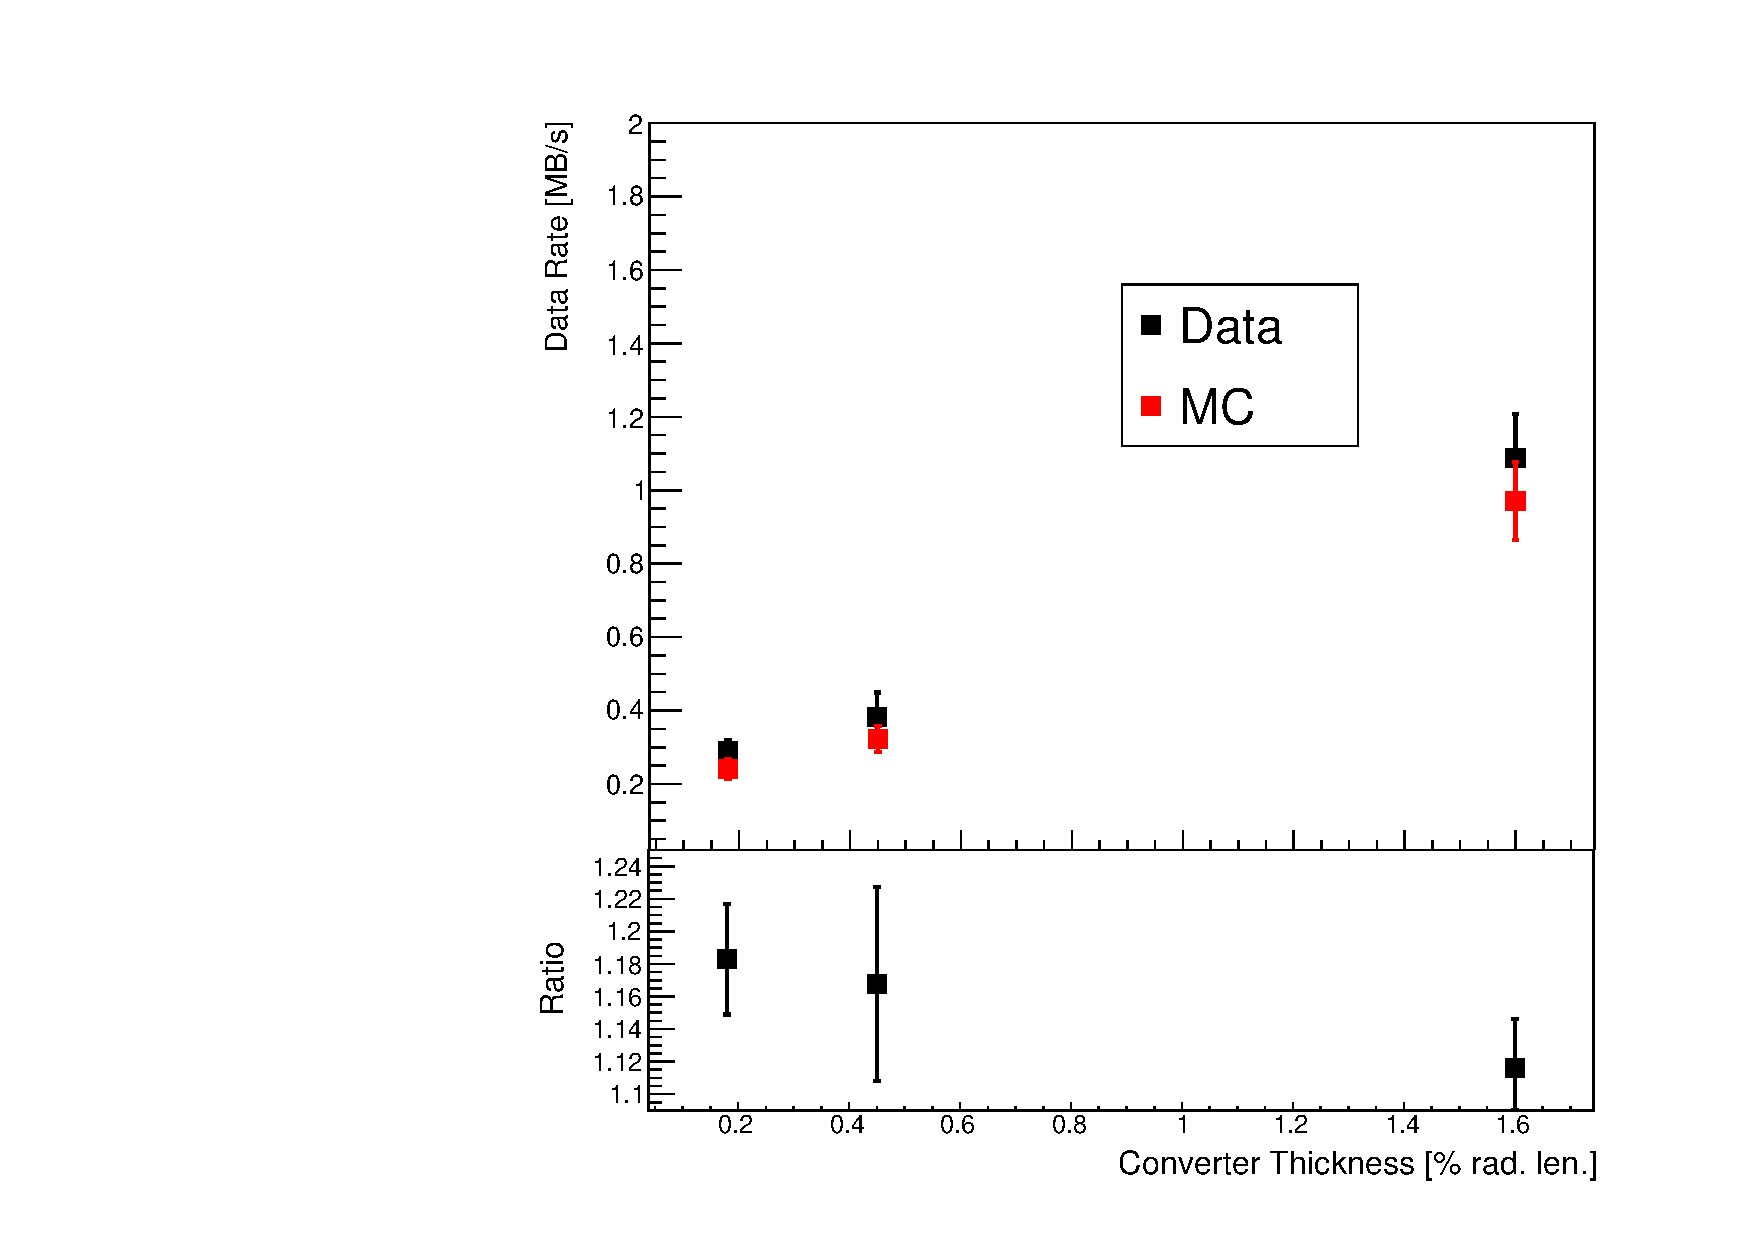
\includegraphics[width=0.49\textwidth]{test2012/svtperformance/daq/data_rate_vs_target_thick.pdf}
        \caption{ { \small
                    Comparison of SVT occupancy between test run data (before and after masking noisy channels) and that expected from simulation.
                } }
	\label{fig:data_rates_data_mc_cmp}
\end{figure}
Similarly, the hit efficiency was measured to be above 98\% for known good layers, see Figure~\ref{fig:hit_efficiency}.
\begin{figure}[h]
    	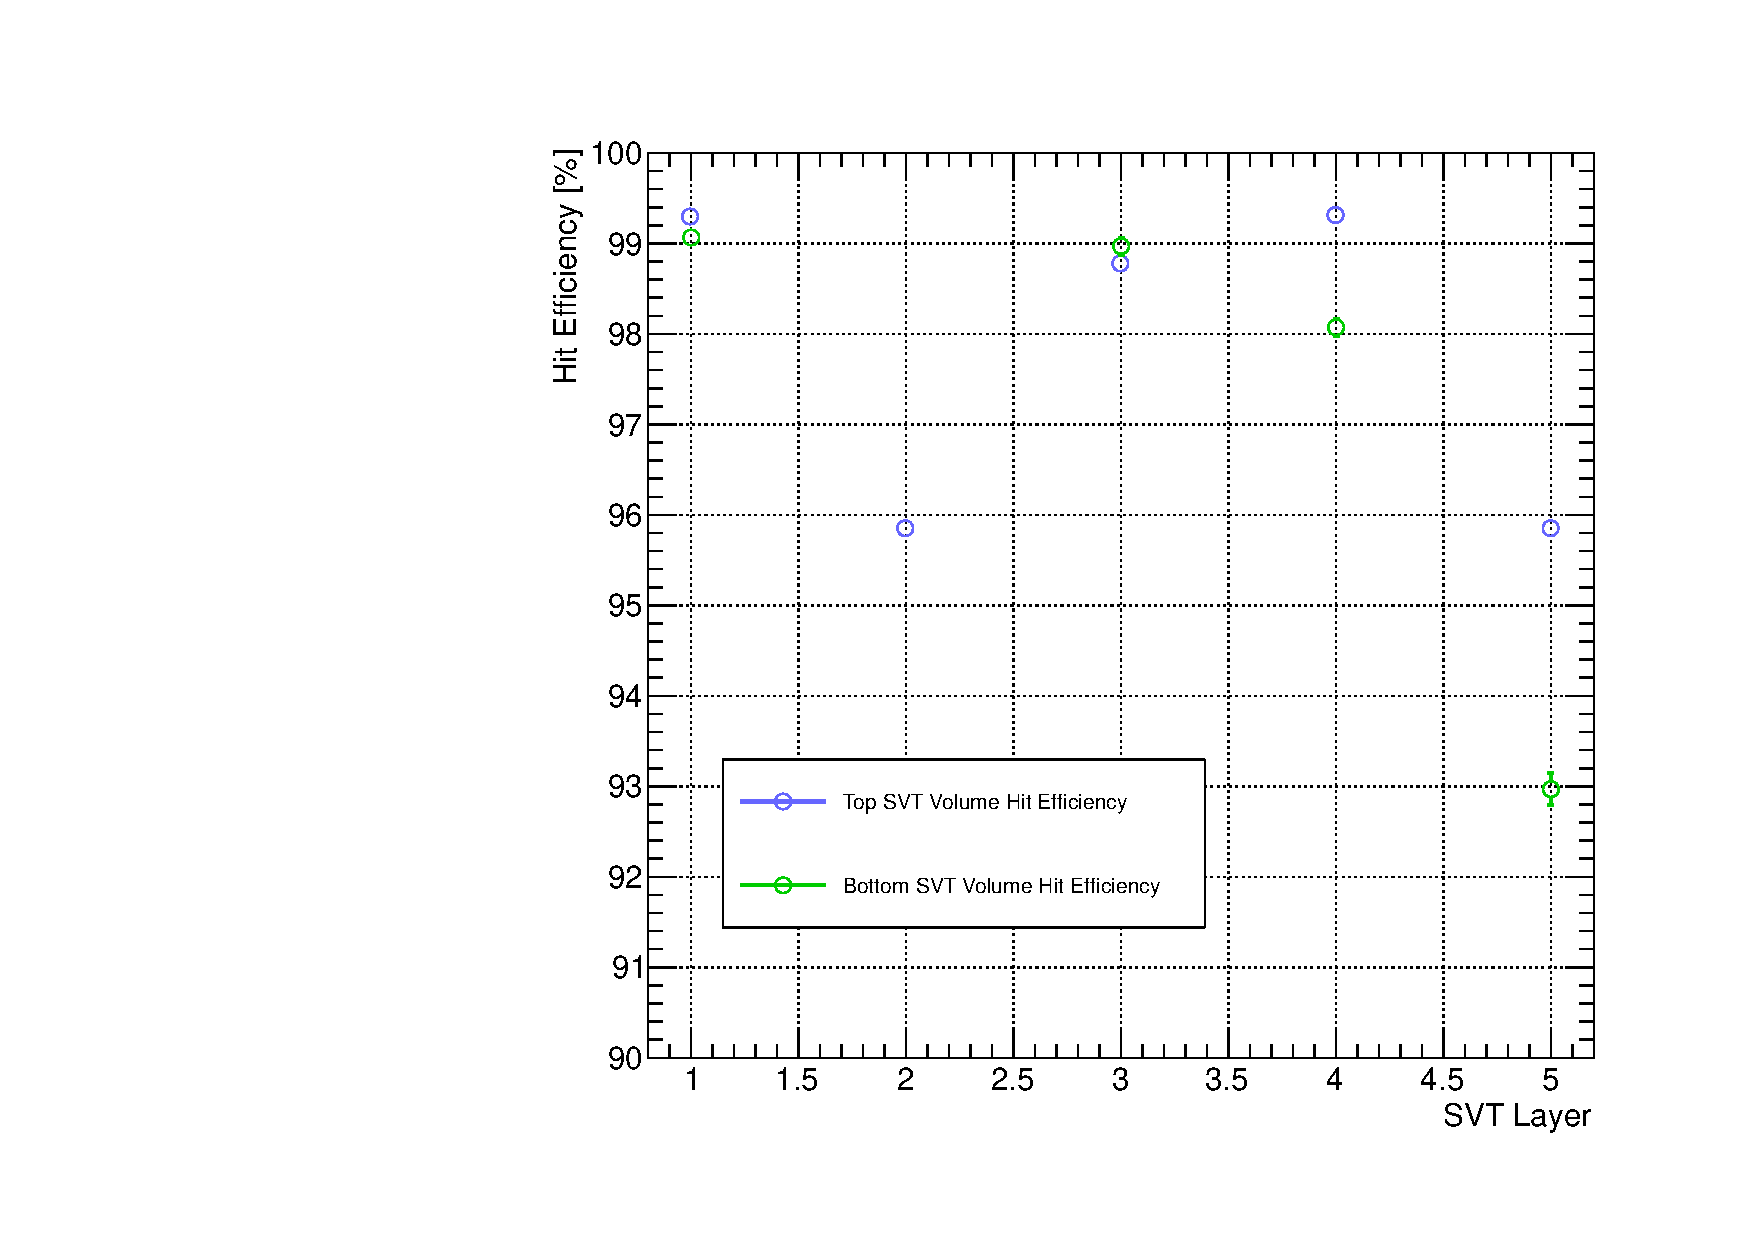
\includegraphics[width=.95\textwidth]{test2012/svtperformance/trk_performance/hit_efficiency_vs_layer.pdf}
%    	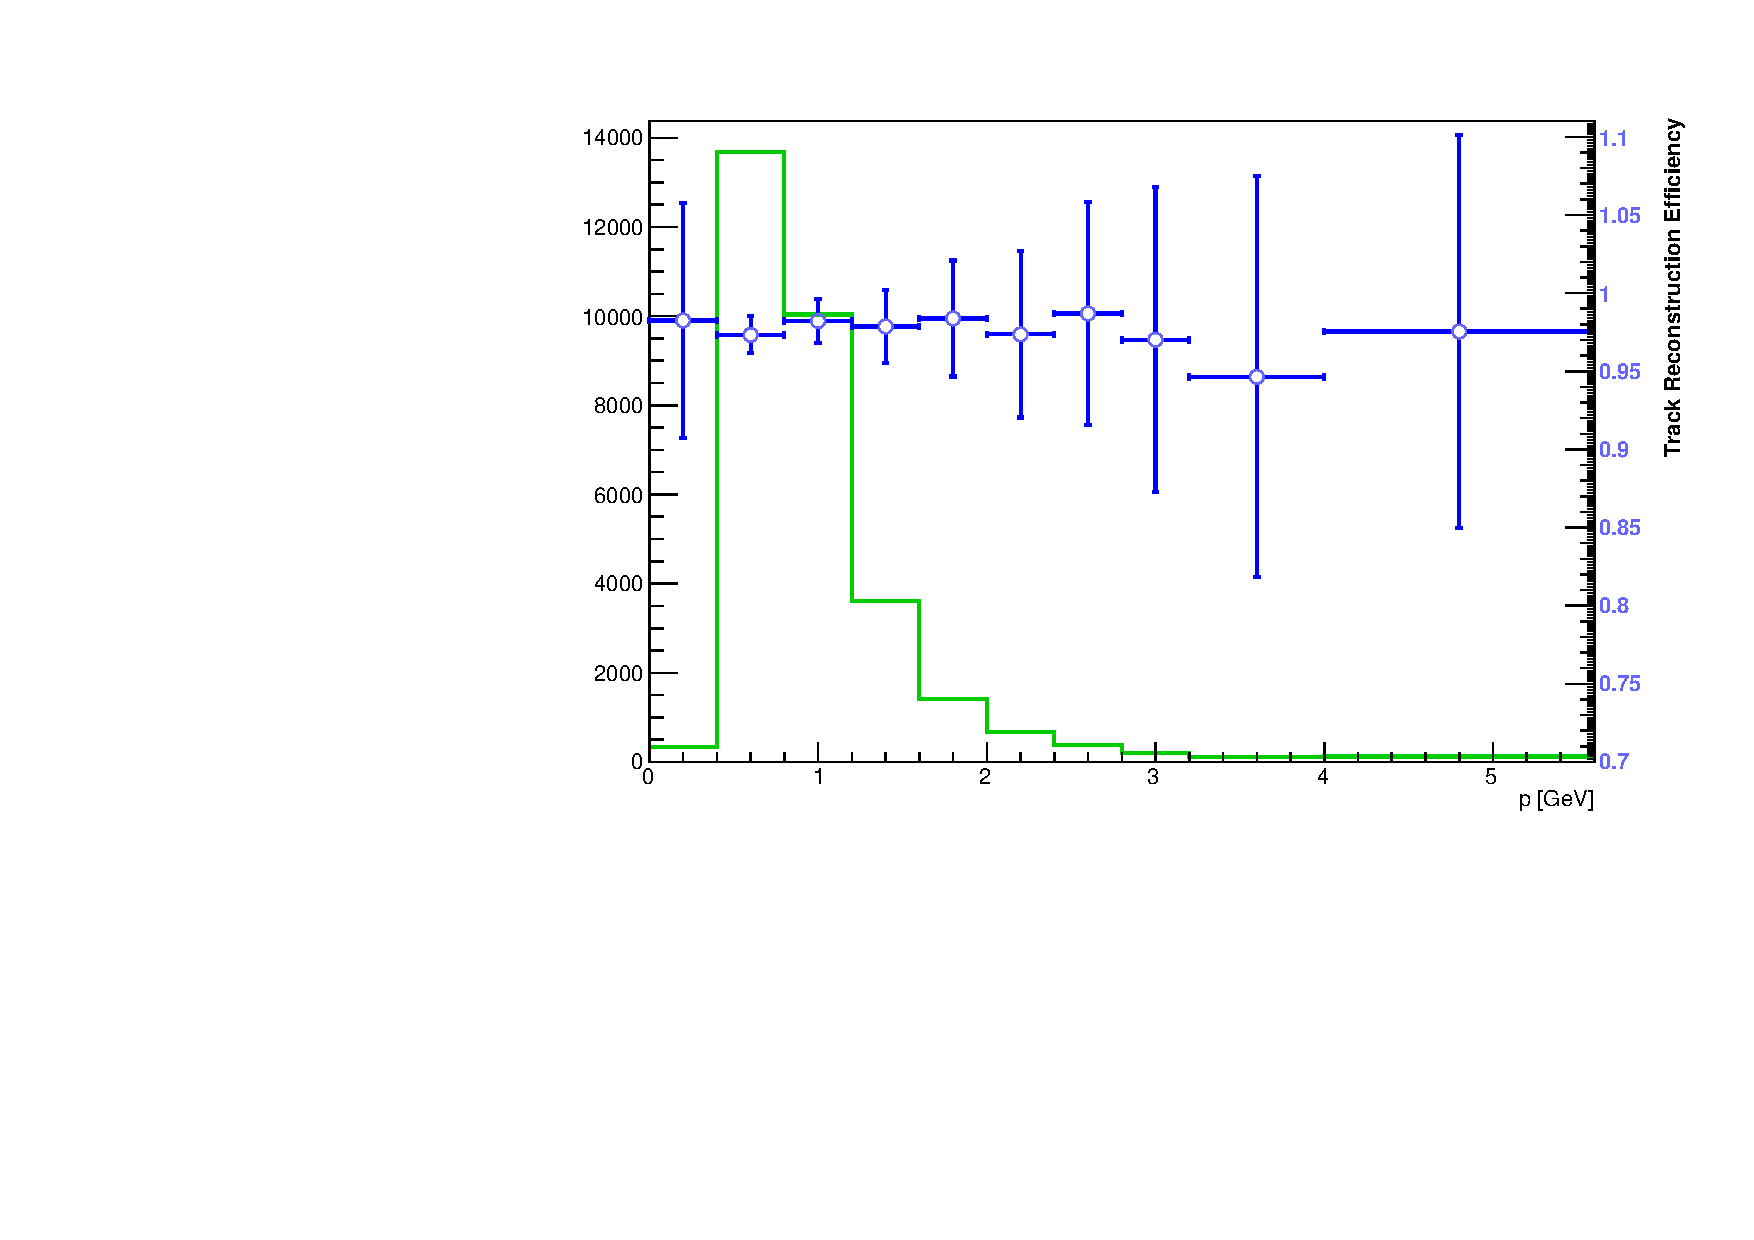
\includegraphics[width=0.49\textwidth]{test2012/svtperformance/trk_performance/track_reco_efficiency.pdf}
        \caption{{\small The hit reconstruction efficiency as a function of detector layer. The variation across the layers can be explained by known DAQ issues.}} 
	\label{fig:hit_efficiency}
\end{figure}
% Further details can be found in the Appendix \ref{app:svt}. 

The spatial resolution of similar microstrip sensors is well established by test beam data, against which the charge deposition model in the lcsim Monte Carlo is validated.  This resolution can be parameterized as a function of the total signal to single-strip noise (S/N) and the crossing angle of tracks through the sensor.  The single-hit resolution for charged particles with $S/N > 20$, as demonstrated here, is relatively constant at approximately 6 $\mu$m for tracks that are close to normal to the sensors as in HPS.

%The spatial resolution of the microstrip sensor discussed in With tracks of only a few GeV multiple scattering prohibits the measurement of spatial hit resolution.  However, as discussed in Sec.~\ref{sec:svt_testrun} the 
%spatial resolution of the microstrip tracker depends mostly on the signal to noise ratio. The measured signal 
%to noise ratio in the test run detector indicates a spatial hit resolution as predicted.

All events containing pairs of oppositely charged tracks were fit to a
common vertex using a simple vertexing algorithm which searches for the distance
of closest approach between the two tracks.  The reconstructed vertex position
along the beam axis for both data and Monte Carlo is shown on 
Figure~\ref{fig:vz_position}.
\begin{figure}[h]
    \begin{center}
    	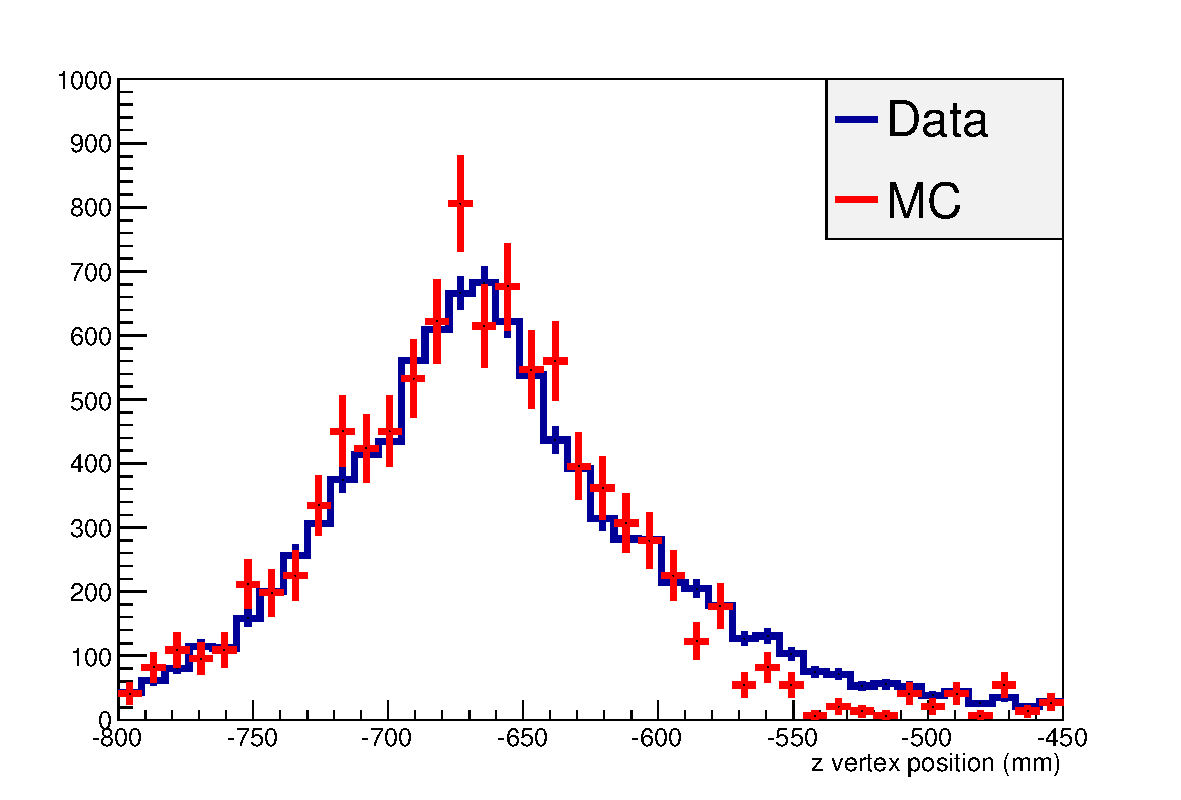
\includegraphics[width=0.60\textwidth]{test2012/svtperformance/trk_performance/zvertex.pdf}
        \caption{  
                    The reconstructed vertex position along the beam axis for
                    both data (blue) and Monte Carlo (red).
                } 
	\label{fig:vz_position}
    \end{center}
\end{figure}
The positioning of the test run SVT layers was such that observation of pairs produced by
the incident photon required both electrons to experience a hard scatter
within the target.  This results in a broadening of the Gaussian 
distributed reconstructed vertex position. 